\section{DBSCAN}
DBSCAN \cite{dbscan} jest popularnym algorytmem grupowania gęstościowego. Najważniejsze jego zalety wymienione przez autorów to tworzenie grup o dowolnym kształcie oraz możliwość doboru parametrów przy niewielkiej wiedzy o zbiorze danych. Grupy tworzone są na podstawie lokalnej gęstości punktu rozumianej jako liczba punktów w tzw. $ \varepsilon $-otoczeniu punktu i mają intuicyjne kształty. Ważną cechą DBSCAN jest też pojęcie punktów szumu, czyli takich, które nie pasują do żadnej grupy. Punkty szumu mogą być cenne, na przykład przy wykrywaniu anomalii.

\subsection{Definicje}
Zakładam, że grupowaniu poddany jest zbiór punktów \s{D} i wartości $ \varepsilon $, $ \mu $ są ustalone.
\smallskip

\definition{\s{d:eps-otoczenie} (ang. $ \varepsilon $-neighbourhood)}\newline
 Zbiór punktów $ V \subseteq \s{D} $ jest $ \varepsilon $-otoczeniem punktu $ p\in D $ ($ \s{N}_{D,\varepsilon}(p) $), jeśli każdy punkt $ q \in V $ znajduje się w odległości nie większej niż $ \varepsilon $ od punktu $ p $.
\begin{equation}\label{eq:eps-neighbourhood}
	\s{N}_{D,\varepsilon}(p) = \set{q \in D | \s{d}(p, q) \le \varepsilon} \land p \in D
\end{equation}

\definition{\s{d:punkt rdzeniowy} (ang. core point) (\myhyperref{fig:core-edge-point}{rysunek})}\newline
Punkt $ p \in D $ jest punktem rdzeniowym ($ core_{D,\varepsilon,\mu}(p) $), jeśli liczba punktów w $ \varepsilon $-otoczeniu punktu $ p $ jest większa lub równa $ \mu $.

\begin{equation}\label{core-point}
	\s{core}_{D,\varepsilon,\mu}(p) \iff |N_{D,\varepsilon}(p)| \ge \mu \land p \in D
\end{equation}

\begin{figure}
	\centering
  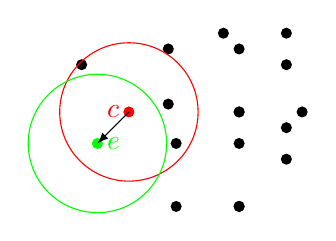
\begin{tikzpicture}
		\fill (-2,1.8) circle(2pt);
		\fill (-.9, 1.3) circle(2pt);
		\fill (-.9,2) circle(2pt);
		\fill (-.8,.8) circle(2pt);
		\fill (-.8,0) circle(2pt);
		\fill (-.2,2.2) circle(2pt);
		\fill (0,0) circle(2pt);
		\fill (0,1.2) circle(2pt);
		\fill (0,1.2) circle(2pt);
		\fill (0,0) circle(2pt);
		\fill (0,.8) circle(2pt);
		\fill (0,2) circle(2pt);
		\fill (.6,1) circle(2pt);
		\fill (.6,.6) circle(2pt);
		\fill (.6,1.8) circle(2pt);
		\fill (.6,2.2) circle(2pt);
		\fill (.8,1.2) circle(2pt);
    
    \fill[red] (-1.4,1.2) circle(2pt) node[anchor=east]{$ c $};
    \draw[red] (-1.4,1.2) circle(25pt);
    
    \fill[green] (-1.8,.8) circle(2pt) node[anchor=west]{$ e $};
    \draw[green] (-1.8,.8) circle(25pt);
    
		\draw[-latex] (-1.4,1.2) -- (-1.8,.8);
		
  \end{tikzpicture}
  \caption{Punkt rdzeniowy $ c $, brzegowy $ e $ oraz relacja bezpośredniej gęstościowej osiągalności $ dirreach_{\varepsilon,\mu}(e, c) $, $ \mu=3$.}\label{fig:core-edge-point}
\end{figure}

\definition{\s{d:dirreach} (ang. direct density reachability) (\myhyperref{fig:core-edge-point}{rysunek})}\newline
Punkt $ p \in D $ jest bezpośrednio gęstościowo osiągalny z punktu $ q \in D $ ($ dirreach_{D,\varepsilon,\mu}(p, q) $), jeśli $ q $ jest punktem rdzeniowym i $ p $ należy do $ \varepsilon $-otoczenia punktu $ q $.
\begin{equation} \label{direct-reachability}
	\s{dirreach}_{D,\varepsilon,\mu}(p, q) \iff p \in N_{D,\varepsilon}(q) \land core_{D,\varepsilon,\mu}(q)
\end{equation}
To, że $ p $ jest bezpośrednio gęstościowo osiągalny z $ q $, nie implikuje, \mbox{że $ q $ jest} bezpośrednio gęstościowo osiągalny z $ p $. Własność ta może być wyrażona następująco:
\begin{equation} \label{direct-reachability-asymmetry}
	\exists_D\;\neg\forall_{p,q\in D}\;dirreach_{D,\varepsilon,\mu}(p, q) \implies dirreach_{D,\varepsilon,\mu}(q, p)
\end{equation}

\pagebreak\definition{\s{d:punkt brzegowy} (ang. edge point) (\myhyperref{fig:core-edge-point}{rysunek})}\newline
Punkt $ p \in D $ jest punktem brzegowym ($ \s{edge}_{D,\varepsilon,\mu}(p) $), jeśli nie jest punktem rdzeniowym i jest bezpośrednio gęstościowo osiągalny z innego \mbox{punktu $ q \in D $}.
\begin{equation}\label{edge-point}
	edge_{D,\varepsilon,\mu}(p) \iff \neg core_{D,\varepsilon,\mu}(p) \land \exists_{q\in D}\, dirreach_{D,\varepsilon,\mu}(p,q)
\end{equation}

\definition{\s{d:reach} (ang. density reachability) (\myhyperref{fig:density-reachablity-reachability}{rysunek})}\newline
Punkt $ p_1 \in D$ jest gęstościowo osiągalny z punktu $ p_n\in D $ ($ \s{reach}_{D,\varepsilon,\mu}(p_1, p_n) $), jeśli istnieje ciąg punktów $ p_1,\dots,p_n \in D $, taki że każdy punkt tego ciągu, poza ostatnim, jest bezpośrednio gęstościowo osiągalny z punktu następnego.
\begin{equation}
	\exists_{p_1,\dots,p_n\in D}\,\forall_{i\in\set{1,\dots,n-1}}\,dirreach_{D,\varepsilon,\mu}(p_i, p_{i+1}) \implies \s{reach}_{D,\varepsilon,\mu}(p_1, p_n)
\end{equation}

\begin{figure}
	\begin{minipage}[b]{.5\linewidth}
		\centering
		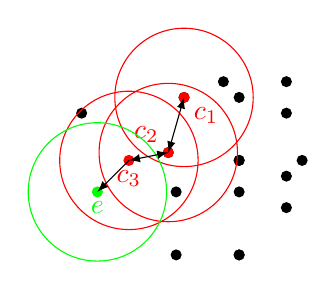
\begin{tikzpicture}
			\fill (-2,1.8) circle(2pt);
			\fill (-.9, 1.3) circle(2pt);
			\fill (-.8,.8) circle(2pt);
			\fill (-.8,0) circle(2pt);
			\fill (-.7,2) circle(2pt);
			\fill (-.2,2.2) circle(2pt);
			\fill (0,0) circle(2pt);
			\fill (0,1.2) circle(2pt);
			\fill (0,1.2) circle(2pt);
			\fill (0,0) circle(2pt);
			\fill (0,.8) circle(2pt);
			\fill (0,2) circle(2pt);
			\fill (.6,1) circle(2pt);
			\fill (.6,.6) circle(2pt);
			\fill (.6,1.8) circle(2pt);
			\fill (.6,2.2) circle(2pt);
			\fill (.8,1.2) circle(2pt);
			
			\fill[red] (-.7, 2) circle(2pt) node[anchor=north west]{$ c_1 $};
			\draw[red] (-.7, 2) circle(25pt);
			
			\fill[red] (-.9, 1.3) circle(2pt) node[anchor=south east]{$ c_2 $};
			\draw[red] (-.9, 1.3) circle(25pt);
			
			\fill[red] (-1.4,1.2) circle(2pt) node[anchor=north]{$ c_3 $};
			\draw[red] (-1.4,1.2) circle(25pt);
			
			\fill[green] (-1.8,.8) circle(2pt) node[anchor=north]{$ e $};
			\draw[green] (-1.8,.8) circle(25pt);
			
			\draw[latex-latex] (-.7, 2) -- (-.9, 1.3);
			\draw[latex-latex] (-.9, 1.3) -- (-1.4,1.2);
			\draw[-latex] (-1.4,1.2) -- (-1.8,.8);
		\end{tikzpicture}
		\subcaption{$ reach_{\varepsilon,\mu}(e, c_1) $} \label{fig:density-reachablity-reachability}
	\end{minipage}
	\begin{minipage}[b]{.5\linewidth}
		\centering
		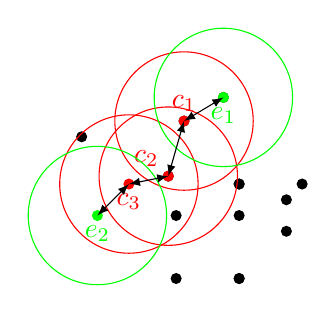
\begin{tikzpicture}
			\fill (-2,1.8) circle(2pt);
			\fill (-.9, 1.3) circle(2pt);
			\fill (-.8,.8) circle(2pt);
			\fill (-.8,0) circle(2pt);
			\fill (-.7,2) circle(2pt);
			\fill (-.2,2.3) circle(2pt);
			\fill (0,0) circle(2pt);
			\fill (0,1.2) circle(2pt);
			\fill (0,1.2) circle(2pt);
			\fill (0,0) circle(2pt);
			\fill (0,.8) circle(2pt);
			\fill (.6,1) circle(2pt);
			\fill (.6,.6) circle(2pt);
			\fill (.8,1.2) circle(2pt);
			
			\fill[red] (-.7, 2) circle(2pt) node[anchor=south]{$ c_1 $};
			\draw[red] (-.7, 2) circle(25pt);
			
			\fill[red] (-.9, 1.3) circle(2pt) node[anchor=south east]{$ c_2 $};
			\draw[red] (-.9, 1.3) circle(25pt);
			
			\fill[red] (-1.4,1.2) circle(2pt) node[anchor=north]{$ c_3 $};
			\draw[red] (-1.4,1.2) circle(25pt);
			
			\fill[green] (-1.8,.8) circle(2pt) node[anchor=north]{$ e_2 $};
			\draw[green] (-1.8,.8) circle(25pt);
			
			\fill[green] (-.2,2.3) circle(2pt) node[anchor=north]{$ e_1 $};
			\draw[green] (-.2,2.3) circle(25pt);
			
			\draw[latex-latex] (-.2,2.3) -- (-.7, 2);
			\draw[latex-latex] (-.7, 2) -- (-.9, 1.3);
			\draw[latex-latex] (-.9, 1.3) -- (-1.4,1.2);
			\draw[latex-latex] (-1.4,1.2) -- (-1.8,.8);
		\end{tikzpicture}
		\subcaption{$ connected_{\varepsilon,\mu}(e_1, e_2) $} \label{fig:density-reachablity-connection}
	\end{minipage}
	\caption{Relacje zasięgu gęstościowego \subref{fig:density-reachablity-reachability} i łączności gęstościowej \subref{fig:density-reachablity-connection}, $ \mu = 3 $.}
\end{figure}

\definition{\s{d:grupa} (ang. cluster)}\newline
Zbiór punktów $ C $ jest grupą w zbiorze punktów $ D $, jeśli zawiera się w $ D $ i jest zbiorem wszystkich punktów gęstościowo osiągalnych z dowolnego punktu rdzeniowego. 
\begin{equation}\label{eq:cluster-def}
C = \set{p \in D | \s{reach}_{D,\varepsilon,\mu}(p, q)} \land core_{D,\varepsilon,\mu}(q)
\end{equation}

\definition{\s{d:punkt szumu} (ang. noise point)}\newline
Punkt $ p\in D $ jest punktem szumu ($ \s{noise}_{D,\varepsilon,\mu}(p) $), jeśli nie jest punktem rdzeniowym oraz nie jest bezpośrednio gęstościowo osiągalny z żadnego punktu $q \in D$. 
\begin{equation}
	noise_{D,\varepsilon,\mu}(p) \iff \neg core_{D,\varepsilon,\mu}(p) \land \forall_{q\in D}\,\neg dirreach_{D,\varepsilon,\mu}(p, q) \land p \in D
\end{equation}

\subsection{Algorytm grupowania}
Na podstawie przedstawionej wcześniej definicji grupy autorzy DBSCAN zaproponowali algorytm grupowania. Wersję tego algorytmu z drobną poprawką prezentuje \myhyperref{alg:dbscan}{algorytm}. Dzięki wprowadzonej poprawce, $ \varepsilon $-otoczenie jest wyznaczane dla każdego punktu tylko raz jak to zaproponowano w \cite{fasterdbscan}, w odróżnieniu od oryginalnej propozycji \cite{dbscan}, gdzie $ \varepsilon $-otoczenie może być wyznaczone więcej niż jeden raz dla tego samego punktu. Dalej nazwa DBSCAN będzie używana w odniesieniu do \myhyperref{alg:dbscan}{algorytmu}.

Okazuje się, że zgodnie z definicją grupy (\myhyperref{eq:cluster-def}{wyrażenie}) punkt $ p $ zbioru danych $ D $ może jednocześnie należeć do więcej niż jednej grupy. Taka sytuacja może mieć miejsce, gdy punkt $ p $ jest gęstościowo osiągalny z punktów rdzeniowych $ q $ i $ r $, ale punkt $ q $ nie jest gęstościowo osiągalny z punktu $ r $. Wtedy punkt $ p $ będzie jednocześnie należał do dwóch różnych grup \mbox{$ C_1 $ oraz $ C_2 $}.
\begin{equation}
  reach_{D,\varepsilon,\mu}(p, q) \land reach_{D,\varepsilon,\mu}(p, r) \land 
  \neg reach_{D,\varepsilon,\mu}(q, r) \implies
  p \in C_1 \cap C_2
\end{equation}
Stąd wynika, że punkt $ p $ musi być punktem brzegowym, ponieważ gdyby był punktem rdzeniowym, to punkt $ q $ byłby gęstościowo osiągalny z punktu $ r $ za pośrednictwem $ p $.

Algorytm DBSCAN przypisuje każdy punkt zbioru danych do odpowiedniej grupy lub do zbioru punktów szumu poprzez nadanie punktom właściwych etykiet. Każdemu punktowi jest przypisywana tylko jedna etykieta, więc punkt może należeć do co najwyżej jednej z grup uzyskanych przy użyciu algorytmu DBSCAN, stąd tworzone grupy nie są ściśle zgodne z definicją grupy (\myhyperref{eq:cluster-def}{wyrażenie}). Punkty brzegowe, które zgodnie z definicją grupy powinny należeć do więcej niż jednej grupy, są przez algorytm DBSCAN przypisywane tylko do jednej z tych grup. Co więcej, to, do której \mbox{z grup} zostanie przypisany punkt brzegowy, zależy od kolejności przetwarzania punktów zbioru danych.

Warto zwrócić uwagę, że $ \varepsilon $-otoczenie może być wyznaczane za pomocą dowolnej miary odległości lub podobieństwa\footnote{w przypadku miary podobieństwa należy w \myhyperref{eq:eps-neighbourhood}{wyrażeniu} zanegować wartość miary lub odwrócić znak nierówności}. Do najczęściej stosowanych miar należą: odległość euklidesowa, odległość Manhattan oraz podobieństwo kosinusowe.
\smallskip

\definition{\s{d:deuklides} (\s{d_e})}
\begin{equation}
	d_e(p, q) = \sqrt{p \cdot q}
\end{equation}
\definition{\s{d:dmanhattan} (\s{d_m})}
\begin{equation}
d_m(p, q) = \sum_i^{n}{\abs{p_i-q_i}} \;:\; p,q\in \mathcal{R}^n
\end{equation}
\definition{\s{d:scos} (\s{s_{cos}})}
\begin{equation}
s_{cos}(p, q) = \frac{p \cdot q}{\norm{p}\norm{q}}
\end{equation}

\begin{algorithm}
 	\caption{DBSCAN \cite{dbscan}}\label{alg:dbscan}

	\DontPrintSemicolon
	
	\SetKwFunction{dbscan}{dbscan}
	\SetKwFunction{expand}{expandcluster}
	
	\setcounter{AlgoLine}{0}
	\nonl\SetKwProg{myproc}{Wejście}{}{}
	\myproc{}{
		$D$ - zbiór danych \;
		$\varepsilon $ - promień otoczenia \;
		$\mu $ - próg liczności otoczenia \;
	}
	\setcounter{AlgoLine}{0}
	\nonl\SetKwProg{myproc}{Wyjście}{}{}
	\myproc{}{
		każdy punkt zbioru $ D $ ma przypisaną etykietę grupy lub szumu\;
	}
	
	
	\setcounter{AlgoLine}{0}
	\nonl\SetKwProg{myproc}{Definicje}{}{}
	\myproc{}{
		$ nextcid() $ - zwraca nową unikalną etykietę grupy\;
		$ noise $ - etykieta szumu\;
		$ unde\f{}ined $ - nieokreślona etykieta\;
		$ cid(v) $ - etykieta punktu $ v $\;
		$ N_{V,\varepsilon}(v) $ - $ \varepsilon $-otoczenie punktu $ v $ w zbiorze $ V $ (\myhyperref{eps-neighbourhood}{wyrażenie})\;
		$ any(V) $ - dowolny element zbioru $ V $\;
		$ core_{V,\varepsilon,\mu}(v) $ - $ v $ jest punktem rdzeniowym w $ V $(\myhyperref{core-point}{wyrażenie})\;
	}
	\nonl\SetKwProg{myalg}{Algorytm}{}{}
	\myalg{\dbscan{$D$, $\varepsilon$, $\mu$}}{
		$ cid \gets nextcid() \;$ \tcp*{etykieta grupy}
		\ForEach{v \textbf{in} D}{
			\If{$ cid(v) = unde\f{}ined $}{
				\lIf{\expand{D, v, cid, $ \varepsilon $, $ \mu $}}{
					$ cid \gets nextcid() $
				}
			}
		}
	}
	\setcounter{AlgoLine}{0}
	\nonl\SetKwProg{myproc}{Procedura}{}{}
	\myproc{\expand{D, v, cid, $ \varepsilon $, $ \mu $}}{
		$ N_v \gets N_{D,\varepsilon}(v) $\;
		\uIf(\tcp*[f]{$ core_{D,\varepsilon,\mu}(v) $}){$ |N_v| \ge \mu $}{ 
			$ seeds \gets \set{w \in N_v | cid(w) = unde\f{}ined \land w \neq v} $\;
			\lForEach{$ w\ \mathbf{in}\ N_v $}{$ cid(w) \gets cid $}
			\While{$ seeds \neq \emptyset $} {
				$ w \gets any(seeds) $\;
				$ seeds \gets seeds \setminus \set{w} $\;
				$ N_w \gets N_{D,\varepsilon}(w) $\;
				\If($ \mathbf{foreach}\ x\ \mathbf{in}\ N_w $ \tcp*[f]{$ core_{D,\varepsilon,\mu}(w) $}){$ |N_w| \ge \mu $}{%
					\If{$ cid(x)\ \mathbf{in}\ \set{unde\f{}ined, noise} $}{
						\lIf{$ cid(x) = unde\f{}ined $}{$ seeds \gets seeds \cup \set{x} $}	
						$ cid(x) \gets cid $
					}
				}
			}
			\KwRet{true}\;
		}\Else{
			$ cid(v) \gets noise $\;
			\KwRet{false}\;
		}
	}
\end{algorithm}

\subsection{Wydajność}
Najbardziej czasochłonną operacją algorytmu DBSCAN (\myhyperref{alg:dbscan}{algorytm}) jest wyznaczanie $ \varepsilon $-otoczenia punktu. Dla każdego punktu $ \varepsilon $-otoczenie wyznaczane jest co najwyżej raz\footnote{$ \varepsilon $-otoczenie punktu $ p $ jest wyznaczane tylko, jeśli etykieta punktu $ p $ jest nieokreślona, a  po wyznaczeniu $ \varepsilon $-otoczenia zawsze do $ p $ jest przypisywana etykieta}, dlatego jeśli za operację podstawową przyjmiemy wyznaczanie $ \varepsilon $-otoczenia, to w takim sensie złożoność algorytmu będzie liniowa.

Decydująca dla wydajnego działania DBSCAN jest optymalna implementacja wyznaczania $ \varepsilon $-otoczenia. Naiwnym sposobem otrzymania $ \varepsilon $-otoczenia jest sprawdzenie dla każdego punktu w zbiorze danych, czy znajduje się \mbox{w $ \varepsilon $-otoczeniu} punktu, dla którego jest poszukiwane $ \varepsilon $-otoczenie. Wyznaczanie $ \varepsilon $-otoczenia w ten sposób cechuje jednak liniowa złożoność względem liczby punktów w zbiorze danych, co przekłada się na złożoność kwadratową algorytmu DBSCAN. Istnieją metody pozwalające na wydajniejsze znajdowanie $ \varepsilon $-otoczenia i zostaną omówione w kolejnym rozdziale.

Obliczanie wartości miary odległości lub podobieństwa stanowi w przypadku punktów o dużej liczbie wymiarów czasochłonny element wyznaczania $ \varepsilon $-otoczenia. Stosowane zazwyczaj miary wymagają liniowej liczby operacji względem wymiarowości zbioru danych. Wprowadza to liniową zależność czasu wyznaczania $ \varepsilon $-otoczenia od wymiarowości zbioru danych. Zakładając, że w podstawowym wariancie DBSCAN liczba operacji wyznaczania $ \varepsilon $-otoczenia jest kwadratowa względem rozmiaru zbioru danych, to za złożoność obliczeniową grupowania $ n $-wymiarowego zbioru danych $ D $ można przyjąć $ \mathcal{O}(\s{dim}(D)|D|^2) $.